\documentclass[journal,12pt,twocolumn]{IEEEtran}
\usepackage{graphicx}
\usepackage[margin=0.5in]{geometry}
\graphicspath{{./figs/}}{}
\usepackage{amsmath,amssymb,amsfonts,amsthm}
\newcommand{\myvec}[1]{\ensuremath{\begin{pmatrix}#1\end{pmatrix}}}
\usepackage{listings}
\usepackage{watermark}
\usepackage{titlesec}
\usepackage{hyperref}
\let\vec\mathbf
\lstset{
frame=single, 
breaklines=true,
columns=fullflexible
}
\providecommand{\norm}[1]{\left\lVert#1\right\rVert}
\providecommand{\abs}[1]{\left\vert#1\right\vert}
\let\vec\mathbf
%\newcommand{\myvec}[1]{\ensuremath{\begin{pmatrix}#1\end{pmatrix}}}
\newcommand{\mydet}[1]{\ensuremath{\begin{vmatrix}#1\end{vmatrix}}}
\providecommand{\brak}[1]{\ensuremath{\left(#1\right)}}
\providecommand{\lbrak}[1]{\ensuremath{\left(#1\right.}}
\providecommand{\rbrak}[1]{\ensuremath{\left.#1\right)}}
\providecommand{\sbrak}[1]{\ensuremath{{}\left[#1\right]}}
\thiswatermark{\centering \put(0,-110.0){\includegraphics[scale=0.12]{iith.png}} }

\title{\mytitle}
\title{
Matrix Assignment - Conics
}
\author{Adarsh Kumar (FWC22068)}
\begin{document}
\maketitle
\tableofcontents
\bigskip


\section{\textbf{Problem}}
If $a \neq 0$ and the line $ 2bx+3cy+4d = 0$ passess through the point of intersection of the parabolas $ y^2 =4ax$ and $ x^2=4ay$ , then
\linebreak
A) $d^2 + (3b-2c)^2 =0 $ \\ B) $d^2 + (3b+2c)^2 =0 $\\ C) $d^2 + (2b-3c)^2 =0 $ \\D) $d^2 + (2b+3c)^2 =0 $
\\
\section{\textbf{Figure}}
\begin{figure}[h]
    \centering
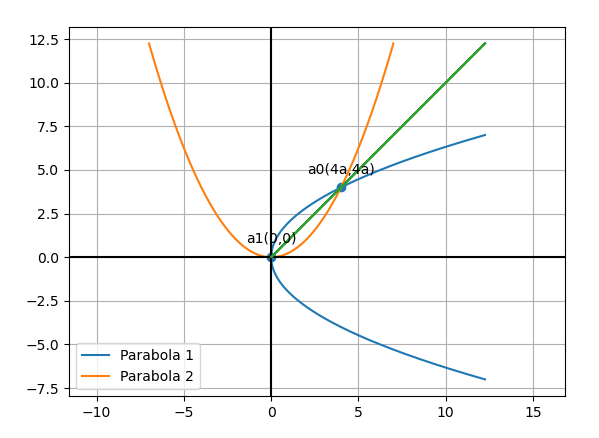
\includegraphics[width=\columnwidth]{con.png}
    \label{fig:my_label}
\end{figure}
\section{\textbf{Solution}}

Let us assume a =1 ;
\textbf{STEP-1}\vspace{2mm}\\
The given equation of parabola $x^2 = 4y$ can be written in the general quadratic form as
\begin{align}
    \vec{x}^{\top}\vec{V}\vec{x}+2\vec{u}^{\top}\vec{x}+f=0
    \end{align}
 
where
\begin{align}
 \vec{V_1} &= \myvec{1 & 0\\0 & 0},
 \label{eq-2-} 
 \\
 \vec{u_1} &= \myvec{0\\-2},
 \label{eq-3-} 
 \\
 f_1 &= 0
 \label{eq-4-} 
 %\\
\end{align}
\\
And also for second Parabola,\\
The given equation of parabola $y^2 = 4x$ can be written in the general quadratic form as
\begin{align}
    \label{eq:conic_quad_form}
    \vec{x}^{\top}\vec{V}\vec{x}+2\vec{u}^{\top}\vec{x}+f=0
    \end{align}
where
\begin{align}
 \vec{V_2} &= \myvec{0 & 0\\0 & 1},
 \label{eq-6-} 
 \\
 \vec{u_2} &= \myvec{-2\\ 0},
 \label{eq-7-} 
 \\
 f_2 &= 0
 \label{eq-8-}  
 %\\
\end{align}
\\
\textbf{STEP-2}\vspace{2mm}\\
The intersection of the given conics is obtained
as\\
\begin{align}
	\vec{x}^{\top}\brak{\vec{V}_1 + \mu\vec{V}_2}\vec{x}+2 \brak{\vec{u}_1+\mu \vec{u}_2}^{\top} \vec{x} 
	+ \brak{f_1+\mu f_2}= 0
	\\
    \end{align}
    
\begin{align}
\vec{V}_1+\mu\vec{V}_2= \myvec{
1 & 0\\
0 & \mu
}
\label{eq-11-}  
\end{align}
\begin{align}
\vec{u}_1+\mu\vec{u}_2= -\myvec{
2 \mu\\
2
}
\label{eq-12-}  
\end{align}
\begin{align}
f_1+\mu f_2= 0
\label{eq-13-}  
\end{align}
This conic is a single straight line if and only if, \\ \vspace{1mm}
\begin{align}
\mydet{\vec{V}_1 + \mu\vec{V}_2 & \vec{u}_1+\mu \vec{u}_2\\ \brak{\vec{u}_1+\mu \vec{u}_2}^{\top} & f_1 + \mu f_2} &= 0
\label{eq-14-}  
\end{align}
And,\\
\begin{align}
\mydet{\vec{V}_1 + \mu\vec{V}_2} & < 0
\end{align}
Substituting \eqref{eq-11-} \eqref{eq-12-} \eqref{eq-13-} in \eqref{eq-14-}\\ \vspace{1mm}
We get,\\ \vspace{1mm}
\begin{align}
\implies \mydet{1& 0 & -2 \mu\\ 
0 & \mu & -2 \\
-2 \mu & -2 & 0
} &= 0
\end{align}
Solving the above equation we get,\\ 
%\begin{align}
%9\mu^3 + 9\mu^2 + 16\mu + 16=0
%\end{align}
\begin{align}
    \mu = -1 ,1
\end{align}
\\
\textbf{case 1 : when $\mu = 1$}\\
So,\\
\begin{align}
\mydet{\vec{V}_1 + \mu\vec{V}_2} & > 0
\end{align}
\\
So, $\mu =1 $ is discarded\\
\textbf{case 2 : when $\mu = -1$}\\
So,\\
\begin{align}
\mydet{\vec{V}_1 + \mu\vec{V}_2} & < 0
\end{align}
\\
\textbf{Therefore $\mu = 1$}\\
 The eigenvalue decomposition of a symmetric matrix $\vec{V}$ is given by
  \begin{equation}
  \vec{P}^{\top}\vec{V}\vec{P} = \vec{D} \hspace{1cm} 
  \label{eq-20-} 
  \vec{P} = \myvec{\vec{P_1} & \vec{P_2}}                                                    
  \end{equation}
\begin{equation}
 \vec{D} = \begin{pmatrix}
          \lambda_1 & 0 \\
          0 & \lambda_2 \\
          \end{pmatrix}
  \end{equation}
  On solving \eqref{eq-20-} with $\vec{P_1} = \myvec{1 \\ 0} \hspace{2mm} \& \hspace{2mm} \vec{P_2} = \myvec{0 \\ 1}$,\\ we get
  \begin{equation}
 \vec{D} = \begin{pmatrix}
         1 & 0 \\                                                                              0 & 1 \\                                                                              
 \end{pmatrix}                                                                      
\end{equation}
where,
  \begin{equation}
  \lambda_1 = 1 \hspace{2mm} and \hspace{2mm} \lambda_2 = 1
  \end{equation}
\\
Now ,
 Normal vector  $\vec{n_1}$ is given by                                              \begin{equation}                                                                    
\vec{n_1} = \vec{P}(\frac{\sqrt{|\lambda_1|}}{\sqrt{|\lambda_2|}} ) = \myvec{1 \\1},
\end{equation}
\\
Now,
 Normal vector  $\vec{n_2}$ is given by                                              \begin{equation}                                                                    
\vec{n_1} = \vec{P}(\frac{\sqrt{|\lambda_1|}}{ - \sqrt{|\lambda_2|}} ) = \myvec{1 \\-1},
\end{equation}
Now ,\\
We know that $C = V^{-1} u $\\
So, 
\begin{align}
\vec{V}_1+\mu\vec{V}_2= \myvec{
1 & 0\\
0 & \-1
}
\end{align}
\\
\begin{align}
\vec{u}_1+\mu\vec{u}_2= \myvec{
2\\
-2
}
\end{align}
\\
So, $\vec{C} = V^{-1} u = \myvec{-2 \\ -2} $
\\
Now ,\\
\begin{align}
\vec{m_1}= {\vec{Omat} } \hspace{1mm} \vec{n_1} = \myvec{1\\ -1}
\end{align}
\\
And,\\
\begin{align}
\vec{m_2}= {\vec{Omat} } \hspace{1mm} \vec{n_2} = \myvec{1\\ 1}
\end{align}
\\
Now,\\
The intersection of line $\vec{l_1}= C + \lambda \vec{m_1}$ has no real solution \\
And,\\
The intersection of line $\vec{l_2}= C + \lambda \vec{m_2}$ is \\
\begin{align}
\myvec{ 0\\0} and \myvec{4 \\4}
\end{align}
\\
So, From the above calculations ,\\
 we can conclude that , the general equation of line is $y=x$\\
 \newpage
The points of intersection of the line 
\begin{equation}
 L: \quad \vec{x} = \vec{q} + \mu \vec{m} \quad \mu \in \mathbf{R}
\label{eq:conic_tangent}
\end{equation}
with the conic section are given by
\begin{equation}
\vec{x}_i = \vec{q} + \mu_i \vec{m}
\label{eq-32-} 
\end{equation}

%
where
{\tiny
\begin{multline}
\mu_i = \frac{1}
{
\vec{m}^T\vec{V}\vec{m}
}
\lbrak{-\vec{m}^T\brak{\vec{V}\vec{q}+\vec{u}}}
\\
\pm
\rbrak{\sqrt{
\sbrak{
\vec{m}^T\brak{\vec{V}\vec{q}+\vec{u}}
}^2
-
\brak
{
\vec{q}^T\vec{V}\vec{q} + 2\vec{u}^T\vec{q} +f
}
\brak{\vec{m}^T\vec{V}\vec{m}}
\label{eq-33-} 
}
}
\end{multline}
\normalsize
From the line y=x the vectors q,m are taken,
\begin{equation}
\vec{q}=\myvec{0\\0}
\label{eq-34-} 
\end{equation}

\begin{equation} \\
\vec{m}=\myvec{1\\1}
\label{eq-35-} 
\end{equation}
\\
\textbf{For Parabola 1},\\

by substituting \eqref{eq-2-} \eqref{eq-3-} \eqref{eq-4-} \eqref{eq-34-} \eqref{eq-35-}  in \hspace{1mm}\eqref{eq-33-}
\begin{equation}
\mu_i=2
\label{eq-36-} 
\end{equation}

substituting \eqref{eq-34-} \eqref{eq-35-} \eqref{eq-36-} in \eqref{eq-32-} ,\\
the intersection points on the parabola are
\begin{equation}
\vec{a_0}=\myvec{4\\4}
\end{equation}
\begin{equation}
\vec{a_1}=\myvec{0\\0} \\ 
\end{equation}\\
\textbf{For parabola 2},
by substituting by substituting \eqref{eq-6-} \eqref{eq-7-} \eqref{eq-8-} \eqref{eq-34-} \eqref{eq-35-}  in \hspace{1mm} \eqref{eq-33-}
\begin{equation}
\mu_i=2
\label{eq-39-} \\ 34,35,39,32
\end{equation}
substituting \eqref{eq-34-} \eqref{eq-35-} \eqref{eq-39-} in \eqref{eq-32-},\\
the intersection points on the parabola are
\begin{equation}
\vec{a_0}=\myvec{4\\4}
\end{equation}
\begin{equation}
\vec{a_1}=\myvec{0\\0}
\end{equation}\\
So, Here we can clearly see that the both the Parabolas are intersecting each other at two points i.e \\
at  $\vec{a_0}=\myvec{4a\\4a}$ and $\vec{a_1}=\myvec{0\\0}$
\\
Now,\\
\textbf{Case 1 :}
As the line $ 2bx+3cy+4d = 0$ passes through the intersection points of both parabola ,\\
So, at $\vec{a_1}=\myvec{0\\0}$
\\
$ 2b(0)+3c(0)+4d = 0$ \\
$ \Rightarrow 4d =0 $ \\
Also , $d = 0$\\
\textbf{Case 2 :}
As the line $ 2bx+3cy+4d = 0$ passes through the intersection points of both parabola ,\\
So, at $\vec{a_0}=\myvec{4a\\4a}$
\\
$ 2b(4a)+3c(4a)+4d = 0$ \\
So,\\
$\Rightarrow 8ab+12ac= 0$  (Since d=0)\\
$\Rightarrow 4a(2b+3c) = 0 $\\
Since $ a\neq 0$ \\
we can write ,,\\
$2b+3c=0$\\
Also ,
$ (2b+3c)^2 = 0$ \\
So,\\
we can also say that ,\\
$ d^2 + (2b+3c)^2 = 0$\\
So we can conclude that option D is the correct option




\section{\textbf{Code Link}}

\begin{lstlisting}
https://github.com/aadrshptel/Fwc_module1/tree/main/Assignments/Matrix%20assignments/Conics/codes
\end{lstlisting}
Execute the code by using the command\\
\textbf{python3 conic.py}



\end{document}